\documentclass[aspectratio=169, 10pt]{beamer}

% --- Idioma e Codificação ---
\usepackage[utf8]{inputenc}
\usepackage[T1]{fontenc}
\usepackage[brazil]{babel}
\usepackage{lmodern}

% --- Pacotes Gráficos e Diagramação ---
\usepackage{graphicx}
\graphicspath{{./}{/home/pedro/hardcore-life/04-recursos/02-areas-recursos/academico/pesquisas/classe-latex-conepe/}{/home/pedro/hardcore-life/04-recursos/99-meta-assets/imagens/}}
\usepackage{booktabs}
\usepackage{tikz}
\usetikzlibrary{shapes,arrows,positioning,calc}
\usepackage{listings}
\usepackage{tcolorbox}
\tcbuselibrary{skins,breakable}
\usepackage{hyperref}

% --- Cores Institucionais do IFF e do CONEPE ---
\definecolor{iffprimary}{RGB}{30, 130, 60}      % Verde Institucional IFF (#1E823C)
\definecolor{iffdark}{RGB}{15, 60, 30}          % Verde Escuro (#0F3C1E)
\definecolor{ifftext}{RGB}{20, 20, 20}          % Texto Principal (#141414)
\definecolor{iffsubtext}{RGB}{90, 90, 90}       % Texto Secundário (#5A5A5A)
\definecolor{iffred}{RGB}{180, 30, 30}          % Vermelho Alerta (#B41E1E)
\definecolor{iffalertbg}{RGB}{255, 238, 238}    % Fundo Alerta Claro
\definecolor{iffgreenlight}{RGB}{238, 252, 240} % Fundo Sucesso Claro
\definecolor{iffblockbg}{RGB}{245, 247, 248}    % Fundo Bloco Neutro
\definecolor{conepeteal}{RGB}{43, 114, 131}     % Tom Teal CONEPE 2026 (#2B7283)
\definecolor{codebg}{RGB}{245, 247, 250}

% --- Configuração de Geometria e Margens do Beamer ---
\setbeamersize{text margin left=0.6cm, text margin right=0.6cm}
\geometry{headheight=2.362cm}

% --- Tema do Beamer ---
\usetheme{Madrid}
\useinnertheme{rectangles}
\setbeamertemplate{navigation symbols}{}

% --- CABEÇALHO INSTITUCIONAL OFICIAL (FOTO INTEIRA DO CONEPE 2026) ---
% Proporção oficial de alta resolução (2046x302 -> 16.0cm x 2.3617cm), estritamente a foto original
\setbeamertemplate{headline}{%
  \ifnum\insertframenumber<16%
    \nointerlineskip%
    
\includegraphics[width=\paperwidth,height=2.3617cm,keepaspectratio]{cabecalho-conepe2026.jpg}%
  \fi%
}

% --- TÍTULO DO SLIDE (FRAMETITLE) ---
\setbeamerfont{frametitle}{size=\normalsize, series=\bfseries}
\setbeamerfont{framesubtitle}{size=\tiny, series=\normalfont}
\setbeamertemplate{frametitle}{%
  \vspace*{0.08cm}%
  \noindent{\usebeamerfont{frametitle}\color{iffprimary}\insertframetitle}%
  \ifx\insertframesubtitle\@empty%
  \else%
    \par\vspace{0.02cm}{\usebeamerfont{framesubtitle}\color{iffsubtext}\insertframesubtitle}%
  \fi%
  \par\vspace*{-0.15cm}%
}

% --- RODAPÉ INSTITUCIONAL COM LINK DE E-MAIL CLICÁVEL ---
\setbeamertemplate{footline}{%
  \ifnum\insertframenumber>1%
    \ifnum\insertframenumber<16%
      {\color{iffprimary}\hrule height 0.8pt width \paperwidth}%
      \nointerlineskip%
      \begin{beamercolorbox}[wd=\paperwidth,ht=2.6ex,dp=1.1ex,leftskip=0.60cm,rightskip=0.60cm]{empty}%
        {\fontsize{7.5}{9}\selectfont\bfseries\href{mailto:pedroiff0@gmail.com}{\color{ifftext}de Andrade, P. H. R., et al.}}%
        \hfill%
        {\fontsize{7.5}{9}\selectfont\bfseries\href{https://phrandrade.com}{\color{ifftext}Classe \LaTeX\ --- CONEPE 2026}}%
        \hfill%
        {\fontsize{7.5}{9}\selectfont\bfseries\color{ifftext}\insertframenumber{} / \inserttotalframenumber}%
      \end{beamercolorbox}%
      \vspace*{1pt}%
    \fi%
  \fi%
}

% --- Cores dos Blocos e Sumário ---
\setbeamercolor{structure}{fg=iffprimary}
\setbeamercolor{section in toc}{fg=iffprimary}
\setbeamercolor{section number projected}{bg=iffprimary,fg=white}
\setbeamercolor{block title}{bg=iffprimary,fg=white}
\setbeamercolor{block body}{bg=iffblockbg,fg=ifftext}
\setbeamercolor{block title alerted}{bg=iffred,fg=white}
\setbeamercolor{block body alerted}{bg=iffalertbg,fg=ifftext}

% --- Configurações de Caixas (tcolorbox) compactas ---
\tcbset{
  top=1.0mm,
  bottom=1.0mm,
  left=2.0mm,
  right=2.0mm,
  boxsep=1.0mm
}

% --- Configurações de Código ---
\lstset{
  basicstyle=\ttfamily\scriptsize,
  keywordstyle=\color{iffprimary}\bfseries,
  commentstyle=\color{gray}\itshape,
  stringstyle=\color{iffred},
  backgroundcolor=\color{codebg},
  frame=single,
  rulecolor=\color{gray!30},
  breaklines=true,
  showstringspaces=false,
  tabsize=2,
  aboveskip=2pt,
  belowskip=2pt
}

% --- Metadados do Trabalho ---
\hypersetup{
  pdftitle={Classe LaTeX: Otimizacao da Formatacao de Trabalhos Academicos - CONEPE 2026},
  pdfauthor={de Andrade, P. H. R., et al.},
  colorlinks=true,
  linkcolor=iffprimary,
  urlcolor=iffprimary,
  citecolor=iffprimary
}

\title[\texttt{ifftese.cls} --- CONEPE 2026]{Classe \LaTeX: Otimização da Formatação de Trabalhos Acadêmicos}
\subtitle{Automação Normativa da ABNT e Abstração Estrutural com \texttt{ifftese.cls} e \texttt{macros.sty}}

\author[de Andrade, P. H. R., et al.]{
  \textbf{Pedro Henrique Rocha de Andrade}\textsuperscript{1*}, Ana Cecília Soja\textsuperscript{1},\\
  Maria Luiza Linhares Dantas\textsuperscript{2}, Antônio Manoel de Oliveira Figueiredo\textsuperscript{1}
}

\institute[IFF / PUC-Chile]{
  \textsuperscript{1}Instituto Federal Fluminense (IFF) \quad$\vert$\quad \textsuperscript{2}PUC-Chile\\[0.1ex]
  \texttt{*pedroiff0@gmail.com}\\[0.3ex]
  \tiny \textbf{Apoio Institucional:} CNPq (Projeto 129985/2025-2) $\vert$ IFF Bom Jesus $\vert$ FAPERJ
}

\date{CONEPE 2026 --- 22 a 24 de Setembro de 2026}

% -----------------------------------------------------------------------------
% DOCUMENTO
% -----------------------------------------------------------------------------
\begin{document}

% --- Slide 1: Capa Oficial ---
{
\setbeamertemplate{footline}{}
\begin{frame}
  \vspace*{-0.50cm}
  \titlepage
\end{frame}
}

% --- Slide 2: Sumário da Apresentação ---
\begin{frame}{Estrutura da Apresentação}
  \vspace{0.10cm}
  \tableofcontents
\end{frame}

% =============================================================================
% SEÇÃO 1: CONTEXTUALIZAÇÃO
% =============================================================================
\section{Contextualização \& O Paradoxo do Pesquisador}

% --- Slide 3: O Pesadelo da Madrugada ---
\begin{frame}{O Pesadelo da Madrugada: A Odisseia no Word}
  \begin{columns}[T]
    \begin{column}{0.49\textwidth}
      \textbf{Cenário das 23h59 (Véspera de Entrega):}
      \begin{itemize}\setlength{\itemsep}{1.5pt}
        \item O orientador pede um acréscimo de 3 linhas na Introdução;
        \item O autor insere o texto e aperta \textit{Enter}...
      \end{itemize}
      \vspace{0.10cm}
      \begin{alertblock}{O Efeito Dominó Catastrófico}
        \scriptsize
        \begin{itemize}\setlength{\itemsep}{1.5pt}
          \item Figuras saltam páginas adiante, gerando vazios;
          \item Legendas se desprendem e ficam órfãs;
          \item Ocorre o clássico: \texttt{"Erro! Indicador..."};
          \item As referências numéricas perdem ordenação.
        \end{itemize}
      \end{alertblock}
    \end{column}

    \begin{column}{0.49\textwidth}
      \begin{tcolorbox}[colback=iffblockbg,colframe=iffprimary,arc=1.5mm,title=\textbf{O Custo Operacional Comprovado}]
        \scriptsize
        \begin{itemize}\setlength{\itemsep}{2.5pt}
          \item Quebras de seção corrompem a paginação;
          \item Margens oscilam sem intervenção;
          \item Sumário desalinha os números de página;
          \item \textbf{Diagnóstico:} Até \textbf{70\% do tempo de escrita} é consumido combatendo a ferramenta, não produzindo ciência.
        \end{itemize}
      \end{tcolorbox}
    \end{column}
  \end{columns}
\end{frame}

% --- Slide 4: O Paradoxo do Pesquisador ---
\begin{frame}{O Paradoxo do Pesquisador Acadêmico}
  \begin{columns}[T]
    \begin{column}{0.48\textwidth}
      \begin{tcolorbox}[colback=iffgreenlight,colframe=iffprimary,arc=1.5mm,title=\textbf{O Objetivo Científico Central}]
        \scriptsize
        \begin{itemize}\setlength{\itemsep}{1.5pt}
          \item Formulação e teste de hipóteses científicas;
          \item Coleta e análise rigorosa de dados empíricos;
          \item Redação concisa e impacto científico;
          \item Contribuição para o avanço da sociedade.
        \end{itemize}
      \end{tcolorbox}
    \end{column}

    \begin{column}{0.48\textwidth}
      \begin{tcolorbox}[colback=iffalertbg,colframe=iffred,arc=1.5mm,title=\textbf{A Realidade Burocrática}]
        \scriptsize
        \begin{itemize}\setlength{\itemsep}{1.5pt}
          \item Medir margem de 3 cm e 2 cm na régua da tela;
          \item Batalhar para ocultar número na capa e resumo;
          \item Repadronizar títulos após perda de estilo;
          \item Reformatar espaçamentos manuais a cada revisão.
        \end{itemize}
      \end{tcolorbox}
    \end{column}
  \end{columns}
  \vspace{0.12cm}
  \centering \scriptsize \textbf{Pergunta norteadora:} \textit{Como blindar o pesquisador sem exigir dele conhecimento avançado em programação?}
\end{frame}

% =============================================================================
% SEÇÃO 2: O APARATO NORMATIVO
% =============================================================================
\section{O Labirinto Normativo: ABNT \& IBGE}

% --- Slide 5: NBR 14724 ---
\begin{frame}{As Normas Regentes I: ABNT NBR 14724}
  \begin{columns}[T]
    \begin{column}{0.48\textwidth}
      \begin{block}{\textbf{Geometria e Margens Estritas}}
        \scriptsize
        \begin{itemize}\setlength{\itemsep}{1.5pt}
          \item \textbf{Anverso:} Esquerda e Topo: \textbf{3 cm}; Direita e Base: \textbf{2 cm}.
          \item \textbf{Verso:} Margens espelhadas para encadernação.
          \item \textbf{Corpo:} Fonte 12; tamanho 10 para citações longas e notas.
        \end{itemize}
      \end{block}
      \vspace{0.08cm}
      \begin{tcolorbox}[colback=iffblockbg,colframe=gray!50,arc=1.5mm]
        \tiny \textbf{Citações Longas (> 3 linhas):} Recuo obrigatório de 4 cm, fonte 10 e entrelinhas simples.
      \end{tcolorbox}
    \end{column}

    \begin{column}{0.48\textwidth}
      \begin{alertblock}{\textbf{A Pegadinha da Paginação}}
        \scriptsize
        \begin{itemize}\setlength{\itemsep}{1.5pt}
          \item Folhas pré-textuais são \textbf{contadas} desde a Folha de Rosto;
          \item Numeração física só é \textbf{impressa a partir da Introdução};
          \item No Word: quebras de seção complexas e propensas a corrupção;
          \item Na \texttt{ifftese.cls}: gerido automaticamente na transição.
        \end{itemize}
      \end{alertblock}
    \end{column}
  \end{columns}
\end{frame}

% --- Slide 6: NBR 6023 e 6027 ---
\begin{frame}{As Normas Regentes II: NBR 6023 e NBR 6027}
  \begin{columns}[T]
    \begin{column}{0.48\textwidth}
      \begin{block}{\textbf{NBR 6023 (Referências)}}
        \scriptsize
        \begin{itemize}\setlength{\itemsep}{1.5pt}
          \item \textbf{Alinhamento:} À margem esquerda (nunca justificado!).
          \item \textbf{Espaçamento:} Simples entre linhas; 1 linha em branco entre referências.
          \item \textbf{Destaque:} Uniforme apenas no título.
          \item \textbf{Chamada:} Autor-data ou numérico estrito.
        \end{itemize}
      \end{block}
    \end{column}

    \begin{column}{0.48\textwidth}
      \begin{block}{\textbf{NBR 6027 (Sumário)}}
        \scriptsize
        \begin{itemize}\setlength{\itemsep}{1.5pt}
          \item \textbf{Identidade Tipográfica:} O sumário espelha com precisão a grafia do texto:
            \begin{itemize}\setlength{\itemsep}{1pt}
              \item 1 SEÇÃO PRIMÁRIA (CAIXA ALTA NEGRITO)
              \item 1.1 Seção Secundária (Caixa Baixa Normal)
            \end{itemize}
          \item \textbf{Alinhamento:} Números ligados por pontilhados contínuos (\texttt{.....}).
        \end{itemize}
      \end{block}
    \end{column}
  \end{columns}
\end{frame}

% --- Slide 7: Tabelas vs Quadros ---
\begin{frame}{Diferenciação Normativa: Tabelas (IBGE) vs. Quadros (ABNT)}
  \begin{columns}[T]
    \begin{column}{0.48\textwidth}
      \begin{tcolorbox}[colback=iffgreenlight,colframe=iffprimary,arc=1.5mm,title=\textbf{Tabelas (Normas do IBGE)}]
        \scriptsize
        \begin{itemize}\setlength{\itemsep}{1.5pt}
          \item Dados predominantemente \textbf{numéricos};
          \item \textbf{Laterais abertas} (sem bordas verticais externas);
          \item Linhas horizontais no topo, cabeçalho e base;
          \item Alimenta a \textbf{Lista de Tabelas} pré-textual.
        \end{itemize}
      \end{tcolorbox}
    \end{column}

    \begin{column}{0.48\textwidth}
      \begin{tcolorbox}[colback=iffalertbg,colframe=iffred,arc=1.5mm,title=\textbf{Quadros (Norma ABNT)}]
        \scriptsize
        \begin{itemize}\setlength{\itemsep}{1.5pt}
          \item Dados \textbf{qualitativos, conceituais ou texto};
          \item \textbf{Totalmente fechado} nos 4 lados com grades;
          \item Divisórias internas completas de células;
          \item Exige obrigatoriamente a \textbf{Lista de Quadros}.
        \end{itemize}
      \end{tcolorbox}
    \end{column}
  \end{columns}
  \vspace{0.08cm}
  \begin{alertblock}{O Erro Típico na Academia}
    \tiny Tratar quadro e tabela como sinônimos gera reprovação formal. A \texttt{ifftese.cls} automatiza a separação através das macros \texttt{\textbackslash inserirtabela} e \texttt{\textbackslash inserirquadro}.
  \end{alertblock}
\end{frame}

% =============================================================================
% SEÇÃO 3: PARADIGMAS DE PROCESSAMENTO
% =============================================================================
\section{Princípio dos Paradigmas: WYSIWYG vs. WYSIWYM}

% --- Slide 8: WYSIWYG vs WYSIWYM ---
\begin{frame}{O Princípio dos Paradigmas: WYSIWYG vs. WYSIWYM}
  \begin{columns}[T]
    \begin{column}{0.48\textwidth}
      \begin{tcolorbox}[colback=iffalertbg,colframe=iffred,arc=1.5mm,title=\textbf{WYSIWYG: Microsoft Word}]
        \scriptsize \textit{"What You See Is What You Get"}
        \begin{itemize}\setlength{\itemsep}{2pt}
          \item Mistura texto, renderização gráfica e geometria;
          \item Algoritmo local 'guloso': editar uma linha no topo quebra páginas seguintes em cascata;
          \item Instabilidade severa em documentos longos.
        \end{itemize}
      \end{tcolorbox}
    \end{column}

    \begin{column}{0.48\textwidth}
      \begin{tcolorbox}[colback=iffgreenlight,colframe=iffprimary,arc=1.5mm,title=\textbf{WYSIWYM: O Sistema \LaTeX}]
        \scriptsize \textit{"What You See Is What You Mean"}
        \begin{itemize}\setlength{\itemsep}{2pt}
          \item Fundamentado por Knuth (1977) e Lamport (1984);
          \item O autor declara semântica; o compilador calcula o leiaute global ótimo;
          \item Algoritmo Knuth-Plass: microtipografia estável via programação dinâmica.
        \end{itemize}
      \end{tcolorbox}
    \end{column}
  \end{columns}
\end{frame}

% --- Slide 9: Por Que o LaTeX ---
\begin{frame}{Por Que o \LaTeX\ é a Resposta (e o dilema da curva inicial)}
  \begin{columns}[T]
    \begin{column}{0.48\textwidth}
      \textbf{As Vantagens Inquestionáveis:}
      \begin{itemize}\setlength{\itemsep}{2pt}
        \item Padrão mundial na física e computação;
        \item Tipografia de equações com rigor estético;
        \item Referências cruzadas confiáveis via \texttt{.aux};
        \item Separação total entre conteúdo e arte-final.
      \end{itemize}
    \end{column}

    \begin{column}{0.48\textwidth}
      \begin{alertblock}{\textbf{A Barreira de Entrada}}
        \scriptsize
        \begin{itemize}\setlength{\itemsep}{2pt}
          \item Curva de aprendizado inicial íngreme;
          \item Dezenas de pacotes gráficos para configurar;
          \item Mensagens de erro de compilação intimidadoras;
          \item Necessidade de adequar classes genéricas à ABNT.
        \end{itemize}
      \end{alertblock}
    \end{column}
  \end{columns}
  \vspace{0.10cm}
  \centering \scriptsize \textbf{A Solução Necessária:} Uma camada de abstração institucional desenvolvida sob medida.
\end{frame}

% =============================================================================
% SEÇÃO 4: A SOLUÇÃO PROPOSTA
% =============================================================================
\section{A Solução Proposta: \texttt{ifftese.cls} e \texttt{macros.sty}}

% --- Slide 10: A Solução IFF ---
\begin{frame}{A Solução Proposta: \texttt{ifftese.cls} e \texttt{macros.sty}}
  \begin{block}{\textbf{Objetivo do Projeto}}
    \tiny Desenvolver uma classe tipográfica oficial e um pacote de extensão para atender a comunidade do Instituto Federal Fluminense, assegurando conformidade estrita à ABNT e preservando a identidade visual local.
  \end{block}
  \vspace{0.06cm}
  \begin{columns}[T]
    \begin{column}{0.48\textwidth}
      \begin{tcolorbox}[colback=white,colframe=iffprimary,arc=1.5mm,title=\textbf{Classe \texttt{ifftese.cls}}]
        \scriptsize
        \begin{itemize}\setlength{\itemsep}{1.5pt}
          \item Gerenciamento de margens e geometria milimétrica;
          \item Geração automática de capas e aprovações;
          \item Cabeçalhos e paginação inteligente;
          \item Base construída sobre o ecossistema \texttt{abntex2}.
        \end{itemize}
      \end{tcolorbox}
    \end{column}

    \begin{column}{0.48\textwidth}
      \begin{tcolorbox}[colback=white,colframe=conepeteal,arc=1.5mm,title=\textbf{Extensão \texttt{macros.sty}}]
        \scriptsize
        \begin{itemize}\setlength{\itemsep}{1.5pt}
          \item Abstração de comandos complexos em linha única;
          \item Diferenciação nativa de tabelas e quadros;
          \item Alimentação automática de listas pré-textuais;
          \item Manipulação segura de contadores pós-textuais.
        \end{itemize}
      \end{tcolorbox}
    \end{column}
  \end{columns}
\end{frame}

% =============================================================================
% SEÇÃO 5: METODOLOGIA E RESULTADOS
% =============================================================================
\section{Resultados Práticos e Validação}

% --- Slide 11: Metodologia ---
\begin{frame}{Metodologia de Desenvolvimento em Três Etapas}
  \centering
  \begin{tikzpicture}[node distance=2.2cm, auto, >=latex]
    \tikzstyle{block} = [rectangle, draw=iffprimary, fill=iffgreenlight, text width=3.6cm, text centered, rounded corners, minimum height=0.95cm, font=\scriptsize\bfseries]
    \tikzstyle{line} = [draw, -latex', thick, iffprimary]

    \node [block] (step1) {1. Mapeamento Normativo\\{\tiny NBR 14724, 6023, 6027 e IBGE}};
    \node [block, right of=step1, xshift=2.0cm] (step2) {2. Construção das Macros\\{\tiny Encapsulamento de ambientes}};
    \node [block, right of=step2, xshift=2.0cm] (step3) {3. Template Unificado\\{\tiny Modelo \texttt{main.tex} institucional}};

    \path [line] (step1) -- (step2);
    \path [line] (step2) -- (step3);
  \end{tikzpicture}

  \vspace{0.25cm}
  \begin{columns}[T]
    \begin{column}{0.32\textwidth}
      \scriptsize \textbf{Ambientes de Teste:}\\TeX Live com motores \texttt{pdflatex} e \texttt{bibtex}.
    \end{column}
    \begin{column}{0.32\textwidth}
      \scriptsize \textbf{Acessibilidade:}\\Compatível com Overleaf, TeXPage e repositórios locais.
    \end{column}
    \begin{column}{0.32\textwidth}
      \scriptsize \textbf{Engenharia de Software:}\\Foco centrado na experiência do usuário final.
    \end{column}
  \end{columns}
\end{frame}

% --- Slide 12: Variáveis e Pré-Texto ---
\begin{frame}[fragile]{Resultados: Variáveis Semânticas e Pré-Texto}
  \begin{columns}[T]
    \begin{column}{0.48\textwidth}
      \textbf{Switches de Configuração (Flags):}
      \begin{itemize}\setlength{\itemsep}{1.5pt}
        \item \verb|\frenteVerso|: Margens simples ou espelhadas;
        \item \verb|\capaiff|: Leiaute institucional oficial;
        \item \verb|\corlink|: Contraste para tela ou impressão;
        \item \verb|\sumarioEscada|: Formatação hierárquica.
      \end{itemize}
      \vspace{0.08cm}
      \textbf{Metadados no Preâmbulo:}
      \begin{itemize}\setlength{\itemsep}{1pt}
        \item \verb|\autor|, \verb|\titulo|, \verb|\orientador|, \verb|\data|.
      \end{itemize}
    \end{column}

    \begin{column}{0.50\textwidth}
      \begin{tcolorbox}[colback=codebg,colframe=iffdark,arc=1.5mm,title=\textbf{Geração com Comandos Únicos}]
        \scriptsize
        O autor não formata a capa manualmente:
        \begin{lstlisting}[language=TeX]
\capa
\contracapa
\folhadeaprovacao
        \end{lstlisting}
        \vspace{0.05cm}
        \textbf{Garantias do Compilador:}
        \begin{itemize}\setlength{\itemsep}{1pt}
          \item Espaçamentos milimétricos da NBR 14724;
          \item Contagem oculta de páginas ativada;
          \item Zero intervenção em arquivos auxiliares.
        \end{itemize}
      \end{tcolorbox}
    \end{column}
  \end{columns}
\end{frame}

% --- Slide 13: Inserção de Figuras ---
\begin{frame}[fragile]{Resultados: Elementos Textuais (\texttt{\textbackslash inserirfigura})}
  \begin{columns}[T]
    \begin{column}{0.48\textwidth}
      \begin{tcolorbox}[colback=iffalertbg,colframe=iffred,arc=1.5mm,title=\textbf{\LaTeX\ Convencional (8--10 linhas)}]
\begin{lstlisting}[language=TeX]
\begin{figure}[htbp]
  \centering
  \caption{Diagrama de Fases}
  \includegraphics[width=0.7\textwidth]{fig.png}
  {\footnotesize Fonte: Autor (2026).}
  \label{fig:fases}
\end{figure}
\end{lstlisting}
        \tiny \textbf{Riscos:} Esquecimento de centralização, inversão de posições, rótulos desacoplados.
      \end{tcolorbox}
    \end{column}

    \begin{column}{0.48\textwidth}
      \begin{tcolorbox}[colback=iffgreenlight,colframe=iffprimary,arc=1.5mm,title=\textbf{Com o \texttt{macros.sty} (1 linha!)}]
\begin{lstlisting}[language=TeX]
\inserirfigura[0.7]{fig.png}
  {Diagrama de Fases}
  {Autor (2026)}{fig:fases}
\end{lstlisting}
        \vspace{0.05cm}
        \scriptsize \textbf{Garantias Automáticas:}
        \begin{itemize}\setlength{\itemsep}{1pt}
          \item Legenda rigorosamente no topo (ABNT);
          \item Fonte tipográfica reduzida no rodapé;
          \item Centralização horizontal padronizada;
          \item Rótulo dinâmico enviado à lista de figuras.
        \end{itemize}
      \end{tcolorbox}
    \end{column}
  \end{columns}
\end{frame}

% --- Slide 14: Tabelas e Quadros ---
\begin{frame}{Resultados: Automação IBGE e Blindagem do Pós-Texto}
  \begin{columns}[T]
    \begin{column}{0.48\textwidth}
      \begin{block}{\textbf{Tabelas e Quadros Parametrizados}}
        \scriptsize
        \begin{itemize}\setlength{\itemsep}{2.5pt}
          \item \textbf{Tabela (IBGE):}\\
            \texttt{\textbackslash inserirtabela[esc]\{arq\}\{leg\}\{fonte\}\{lbl\}}\\
            $\to$ Laterais abertas; alimenta Lista de Tabelas.
          \item \textbf{Quadro (ABNT):}\\
            \texttt{\textbackslash inserirquadro[esc]\{arq\}\{leg\}\{fonte\}\{lbl\}}\\
            $\to$ Moldura fechada; alimenta Lista de Quadros.
        \end{itemize}
      \end{block}
    \end{column}

    \begin{column}{0.48\textwidth}
      \begin{tcolorbox}[colback=white,colframe=conepeteal,arc=1.5mm,title=\textbf{Robustez Pós-Textual}]
        \scriptsize
        \begin{itemize}\setlength{\itemsep}{2.5pt}
          \item \textbf{Apêndices e Anexos:} Transição automática da contagem ($1, 2 \to A, B$);
          \item Preservação da hierarquia do sumário geral;
          \item Suporte a erratas e listagens de equações;
          \item Compatibilização total com o \texttt{abntex2cite}.
        \end{itemize}
      \end{tcolorbox}
    \end{column}
  \end{columns}
\end{frame}

% =============================================================================
% SEÇÃO 6: CONCLUSÕES E FUTURO
% =============================================================================
\section{Conclusões e Desdobramentos Futuros}

% --- Slide 15: Conclusões e Futuro ---
\begin{frame}{Conclusões e Desdobramentos Futuros}
  \begin{block}{\textbf{Conclusões}}
    \scriptsize
    \begin{itemize}\setlength{\itemsep}{1.5pt}
      \item A classe \texttt{ifftese.cls} e o pacote \texttt{macros.sty} cumpriram com pleno êxito a abstração da ABNT e IBGE;
      \item Redução drástica no tempo operacional de formatação e eliminação de falhas formais;
      \item A solução democratiza o rigor do \LaTeX\ no Instituto Federal Fluminense.
    \end{itemize}
  \end{block}

  \vspace{0.08cm}

  \begin{tcolorbox}[colback=conepeteal!10,colframe=conepeteal,arc=1.5mm,title=\textbf{Trabalho em Andamento: Interface Web por Formulários}]
    \scriptsize
    \begin{itemize}\setlength{\itemsep}{1.5pt}
      \item Desenvolvimento de uma plataforma online institucional focada na \texttt{ifftese.cls};
      \item O autor preenche apenas formulários web com metadados e textos das seções;
      \item O servidor compila e entrega o PDF diagramado com perfeição nos bastidores.
    \end{itemize}
  \end{tcolorbox}
\end{frame}

% =============================================================================
% SLIDES FINAIS (PADRÃO ENGENHARIA)
% =============================================================================

% --- Slide 16: Slide Unificado de Agradecimento (Via Láctea Blur) ---
{
\setbeamertemplate{headline}{}
\setbeamertemplate{footline}{}
\usebackgroundtemplate{
\includegraphics[width=\paperwidth,height=\paperheight]{vialactea-blur.jpg}}%
\begin{frame}[plain]
  \vspace*{0.20cm}%
  \centering
  \begin{tcolorbox}[
    colback=black!80,
    colframe=iffprimary,
    arc=3.0mm,
    boxrule=1.2pt,
    width=11.2cm,
    halign=center,
    center
  ]
    \color{white}
    {\Large \textbf{Muito Obrigado!}}\quad---\quad{\normalsize \textbf{Perguntas \& Discussão}}\par\vspace{0.08cm}
    {\scriptsize \color{white!90} \textbf{CONEPE 2026 --- XIII Congresso de Ensino, Pesquisa e Extensão}}\par\vspace{0.10cm}
    {\scriptsize \textbf{Contatos:}\quad \href{mailto:pedroiff0@gmail.com}{\color{iffprimary}\textbf{pedroiff0@gmail.com}} \quad$\vert$\quad \href{mailto:ana.soja@iff.edu.br}{\color{iffprimary}\textbf{ana.soja@iff.edu.br}}}\par\vspace{0.12cm}
    \tcbox[colback=white,colframe=white,arc=2.0mm,boxrule=0pt,top=1mm,bottom=1mm,left=1mm,right=1mm]{%
      
\includegraphics[width=2.5cm,height=2.5cm,keepaspectratio]{qr-code-phrandrade.png}%
    }\par\vspace{0.08cm}
    {\footnotesize \bfseries \href{https://phrandrade.com}{\color{white}https://phrandrade.com}}\par\vspace{0.10cm}
    {\tiny \color{white!75} Apoio Institucional: CNPq (Projeto 129985/2025-2), IFF Bom Jesus, PUC-Chile e FAPERJ}
  \end{tcolorbox}
\end{frame}
}

% --- Slide 17: Slide Final Wallpaper (Via Láctea Sem Blur) ---
{
\setbeamertemplate{headline}{}
\setbeamertemplate{footline}{}
\usebackgroundtemplate{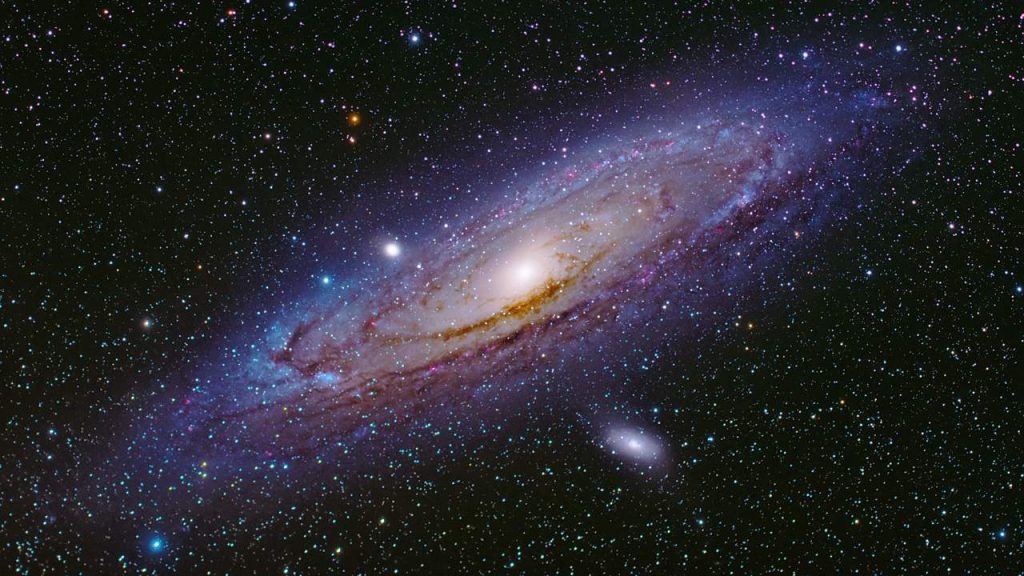
\includegraphics[width=\paperwidth,height=\paperheight]{via-lactea.jpg}}%
\begin{frame}[plain]
\end{frame}
}

\end{document}
